\chapter{Study 3}
\chaptermark{Study 3}
\label{ch:study3}
%\setcounter{equation}{0}

%\newpage
%Abstract
Although the patterns of ongoing thought that make up our day to day lives are important, we know relatively little about how these experiences are constrained by an individuals’ neurocognitive architecture. In the current study we used machine learning to identify stable patterns describing shared variance between performance on a battery of cognitive tasks in the laboratory, and intrinsic neural architecture observed at rest. Next we explored whether these dimensions explained variance in measures of ongoing thought recorded in the laboratory. We identified five neuro cognitive dimensions characterized at the cognitive level as creative association, fluid intelligence, temporally specified cognition, and, separate dimensions of episodic memory linked to visual and verbal codes of representation. Variation in temporally specified cognition - the ability to inhibit a prior mental set during task switching - predicted substantial variance in ongoing experience recorded in the lab, accounting for reduced variance in two principle dimensions identified by PCA---less off task thought and less immersive detail. In neural terms temporally specified cognition was characterized by patterns of high within-network limbic connectivity coupled with relative isolation between this system and other regions of cortex. Together this analysis suggests that whether an individuals thoughts are a pristine representation of the moment, or an immersive experience generated via imagination, depends cognitively on the ability to inhibit prior mental sets, and neurally on the balance of segregation and integration between the limbic system and the rest of the cortex.

% ====================================================================================================================
\section{Introduction}
\label{study3:intro}
Human cognition is not always tethered to the events in the here now. Phenomena such as mind-wandering highlight that we can become immersed in experiences generated from memories, rather than information in the immediate environment \cite{SmallwoodSchooler2015}. Although understanding self-generated experiences may ultimately inform theoretical accounts of both normal cognition and disease states, we currently lack a comprehensive understanding of how these experiences are constrained by an individuals’ neurocognitive architecture.

Contemporary studies have shown that ongoing thought shares important links with both brain and behaviour. For example, the occurrence of off-task thought can jeopardise the integrity of tasks depending on executive control \cite{McVayJOEP2009,MrazekJoEP2012}. On the other hand, states of off task thought and daydreaming can be associated with better performance on tasks of memory and creativity \cite{RubyPlos2013,Poerio2017,WangPsychScience2018,Baird2012}. Neuroimaging studies have highlighted important roles for a number of large scale brain networks \cite<see >[ for meta-analysis]{Fox2015, Stawarczyk2015}. These networks include the default mode network \cite{MasonScience2007,Christoff2009}, the fronto parietal and attention networks \cite{WangNI2018,Golchert2017} and the limbic system \cite{Ellamil2016,Smallwood2016,Golchert2017}.

Associations between patterns of ongoing thought with objective metrics defined from brain and behaviour, raise the possibility that these metrics of individual difference could be used to gain traction on the architecture that underlies patterns of ongoing thought. In the current study, a large cohort of participants (\(n = 197\)) performed a battery of neurocognitive tasks in the laboratory, and, on a separate session we measured their intrinsic brain activity using resting state functional magnetic resonance imaging (fMRI).  These individuals also provided descriptions of their experience while they performed a simple laboratory task across several days.

Using these data we build on our prior work that used canonical correlation analysis (CCA) to reveal neurocognitive dimensions that relate to patterns of ongoing experience \cite{WangPsychScience2018,WangNI2018}. In this study, we used CCA to identify dimensions that linked brain organisation to behaviour, and used these as explanatory variables in analyses predicting patterns of ongoing thought in the laboratory. This allows us to test the view that ongoing thoughts are an emergent property of an individuals’ neural architecture \cite<i.e. >{Gratton2018}.


% ==========================================================================================================

\section{Method}
\label{study3:method}
\subsection{Participants}
\label{study3:method:a}
Two hundred and seven healthy participants were recruited from the University of York (132 females, 65 males; age range = 18–-31 years, \textit{M} = 20.21, \textit{SD} = 2.36).
This analysis included two data sets with some shared measurements and same MRI protocol as chapter \ref{ch:study1}.
Participants were right-handed native English speakers with normal or corrected-to-normal vision and no history of psychiatric or neurological illness. Participants underwent MRI scanning, completed an 1-hr online questionnaire. The first cohort is identical to the sample in chapter\ref{ch:study1}. Participant attended three
(165 participants; 99 females, 66 males; age range = 18–-31 years, \textit{M} = 20.43, \textit{SD} = 2.63) 2-hr behavioral testing sessions to complete a battery of cognitive tasks.
The second cohort (42 participants; 33 females, 9 males; age range = 18–-23 years, \textit{M} = 19.79, \textit{SD} = 1.37) underwent two 2-hr behavioural testing sessions to complete a battery of cognitive tasks. The behavioural sessions took place within a week of the scan. Ten participants were excluded from the multivariate pattern analysis because they failed to complete all of the behavioural testing sessions. In total, 197 participants (126 females, 71 males; age range = 18–-31 years, \textit{M} = 20.11, \textit{SD} = 2.24) were included in the multivariate pattern analysis and the comparison with cognitive performance. Participants were rewarded with either a payment of \pounds 10 per hour or a commensurate amount of course credit. All participants provided written consent prior to the fMRI session and the first behavioural testing session. Approval for the study was obtained from the ethics committee of the University of York Department of Psychology and the University of York Neuroimaging Centre.

\subsection{MRI acquisition}
\label{study3:method:b}
The MRI acquisition protocol was identical to the study documented in chapter \ref{ch:study1}. Please refer to section \ref{study1:method:b} for details.

\subsection{Resting state data preprocessing}
\label{study3:method:c}

All preprocessing and denoising steps for the MRI data were carried out using the SPM software package (Version 12.0) and Conn functional connectivity toolbox (Version 17.f), based on the MATLAB platform (Version 17.a). The first three functional volumes were removed in order to achieve steady state magnetisation. The remaining data was first corrected for motion using six degrees of freedom (x, y, z translations and rotations), and adjusted for differences in slice-time. Subsequently, the high-resolution structural images were co-registered to the mean functional image via rigid-body transformation, segmented into grey/white matter and cerebrospinal fluid probability maps, and all functional volumes were spatially normalized to Montreal Neurological Institute (MNI) space using the segmented images and a priori templates. This indirect procedure utilizes the unified segmentation–normalization framework, which combines tissue segmentation, bias correction, and spatial normalization in a single unified model. No smoothing was employed, complying with recent studies that report the negative influence of this procedure on the construction of connectivity matrices analysis.

Moreover, a growing body of literature indicates the potential influence of participant motion inside the scanner on the subsequent estimates of functional connectivity. To ensure that motion and other artefacts did not confound our data, we have employed an extensive motion-correction procedure and denoising steps, comparable to those reported in the literature. In addition to the removal of six realignment parameters and their second-order derivatives using the general linear model (GLM), a linear detrending term was applied as well as the CompCor method that removed five principle components of the signal from white matter and cerebrospinal fluid. Moreover, the volumes affected by motion were identified and scrubbed based on the conservative settings of motion greater than 0.5 mm and global signal changes larger than z = 3. Though recent reports suggest the ability of global signal regression to account for head motion, it is also known to introduce spurious anti-correlations, and was thus not utilised in our analysis. Finally, a band-pass filter between 0.009 Hz and 0.08 Hz was employed in order to focus on low frequency fluctuations.

\subsection{ROI-ROI functional connectivity.}
\label{study3:method:d}
We adopted a set of 57 regions based on the Yeo 7 networks. We split the networks into two hemispheres and extracted clusters. Two voxels are considered connected only if they are adjacent within the same x, y, or z direction. This yielded 57 clusters from the Yeo 7 networks parcellation. The implementation of spatial clusters extraction was retrieved from python library Nilearn
\cite[ \url{http://nilearn.github.io/}, version 0.3.1]{Abraham2014}.
Fully-connected, undirected and weighted matrices of bivariate correlation coefficients (Pearson's r) were constructed for each participant using the average BOLD signal time series obtained from all the 57 ROIs described above. The off-diagonal of each correlation matrix contained 1596 unique region-region connection strengths (i.e., the upper or lower triangle of the network covariance matrix). This approach provided a measure of connection strength of the whole brain for each participant. Finally, Fisher’s r-to-z transformation was applied to each network covariance matrix.

\subsection{Behavioural data}
\label{study3:method:e}

\subsubsection{Cognitive tasks}
\label{study3:method:e:cog}
We selected 9 cognitive tasks that are common across the two cohorts. The selected tasks measures cognitive functions that have been examined in previous mind-wandering literature, encompassing executive control (digit span, task switching task), generation of information (unusual uses task, verbal fluency task), semantic memory (semantics relatedness judgement tasks, feature matching task), episodic memory (paired associate task, four mountains task), and fluid intelligence (Raven Advanced Progressive Matrices; RAPM). Please refer to Appendix \ref{appendix:study1:subsection2} for the detailed description of the tasks.

Thirteen cognitive scores were calculated from the selected tasks. Performance of the digit span task was represented as the average of digit span in the forward and backward recall conditions. The verbal fluency score is the contrast of the letter condition and the category condition. Picture naming tasks, the four mountains tasks, RAMP were summarised with accuracy scores. The task switching tasks provided two scores (a) flexibility
\footnote{
In the original contrast "switch cost", smaller values indicates better ability to switch away from the previous condition. For the ease of interpretation, we reversed the scores and re-named the contrast as flexibility.}
as the ability to switch from a different condition and (b) inhibition as the ability to suppress information from the previous trial. The calculation of the the task switching contrast can be found in Appendix \ref{appendix:study1:subsection2:TS}. All the semantics related judgement tasks, feature mating task, and the paired associate task were summarised using efficiency scores. The efficiency scores were calculated as reaction time divided by accuracy. A smaller score indicates better performance, thus the scores were reversed to ease the interpretation. For the semantics tasks, we calculated three contrasts based on the semantics modules tested: (a) strength (strong--week) , modality (picture--word), and (c) specificity (specific--general). All the scores were standardised as z-scores in the subsequent analysis.

\subsubsection{Experience sampling}
\label{study3:method:e:mdes}
Multi-dimensional experience sampling (MDES) was use to collect thoughts during a 0-back/1-back working memory task. Please refer to chapter \ref{ch:study1} section \ref{study1:method:d} for the MDES data collection and Table \ref{tab:study1:1} for the detailed questions. The MDES questions were aggregated (a) across all conditions, (b) within the 0-back condition, and (c) within the 1-back condition. All the scores were standardised as z-scores in the subsequent analysis.

\subsection{Multivariate pattern analysis}
\label{study3:method:f}
\subsubsection{SCCA}
We performed a sparse canonical correlation analysis \cite<SCCA; see>{Hastie2015} %{ Hastie, Tibshirani, \& Wainwright, 2015}
on the functional connectomes and the cognitive tasks, to yield latent components that reflect multivariate patterns across neural organisation and cognition \cite<For similar application, see>{WangPsychScience2018}. %Wang et al., 2017).
SCCA maximised the linear correlation between the low-rank projections of two sets of multivatiate data sets with sparse model to regularise the decomposition solutions a process that helps maximise the interpretability of the results. The regularisation function of choice is L1 penalty, which produces ‘sparse’ coefficients, meaning that the canonical vectors (i.e., translating from full variables to a data matrix’s low-rank components of variation) will contain a number of exactly zero elements. L1 regularisation conducted (a) feature selection (i.e., select only relevant components) and (b) model estimation (i.e., determine what combination of components best disentangles the neuro-cognitive relationship) in an identical process. This way we handle adverse behaviours of classical linear models in high-dimensional data. A reliable and robust open-source implementation of the SCCA method was retrieved as R package from CRAN
\cite<PMA, penalized multivariate analysis, version 1.0.9>{Witten2009}. %(PMA, penalized multivariate analysis, version 1.0.9, Witten, Tibshirani, \& Hastie, 2009).
The amount of L1 penalty for the functional connectomes and cognitive task performance were chosen by cross-validation. The procedure is described below.

\subsubsection{Model Selection}
The model selection process was conducted with two parts: L1 penalty coefficient selection and component selection. For the L1 penalty coefficient selection, we performed a grid search combined with cross-validation (CV) to avoid over-fitting \cite{BzdokYeo2017}.
Of each penalty pair on the search grid, a 10-fold cross-validation was performed to search for the best out-of-sample the rank-1 canonical correlation. We then decomposed the full dataset with the selected L1 penalty coefficients. The K-Fold CV was conducted by the implementation in Python library scikit-learn \cite<\url{http://scikit-learn.org/stable/}, version 0.18.2>{scikit-learn}.

Confound removal was performed on the functional connectomes and the cognitive scores as suggested by prior study \cite{Smith2015}.
The confound variables were sex, age, and head motion indicated by mean frame-wise displacement \cite{Jenkinson2002}.
The  removal  steps  was  performed  on  the training set in each CV fold. The z-scores of the confound variables were calculated, and also squared the three confound measures to account for potentially nonlinear effects of these confounds. The 6 resulting confounds were regressed out of both data matrices.
The implementation of the confound removal method \cite{Friston1994} was retrieved from Python library Nilearn \cite[ \url{http://nilearn.github.io/}, version 0.3.1]{Abraham2014}.

After finding the optimal hyper-parameters, 1000 permutation tests with family-wise error correction was applied to access the component(s) that occur above chance. We constructed a null distribution for each canonical component by holding the functional connectivity data in place and randomising the row order of self-reports data. This permutation scheme broke the link of individual differences in the dataset, therefore testing the robustness of the components in the hypothetical population. By calculating the false-discovery rate in the null distribution, we can conclude the possibility of discovering our components by chance with the given penalty coefficients. Hypotheses that are accepted with a 5\% level of significance. In the current analyses we adopt the permutation test with the FWE-corrected p-value by Smith and colleagues \citeyear{Smith2015}. All components were compared to the first sparse canonical correlation of the permuted sample. The low-rank components are more relevant that the rest, therefore we yield more conservative p-value by comparing to the first canonical correlation only.

\begin{figure}[H]
	\centering
	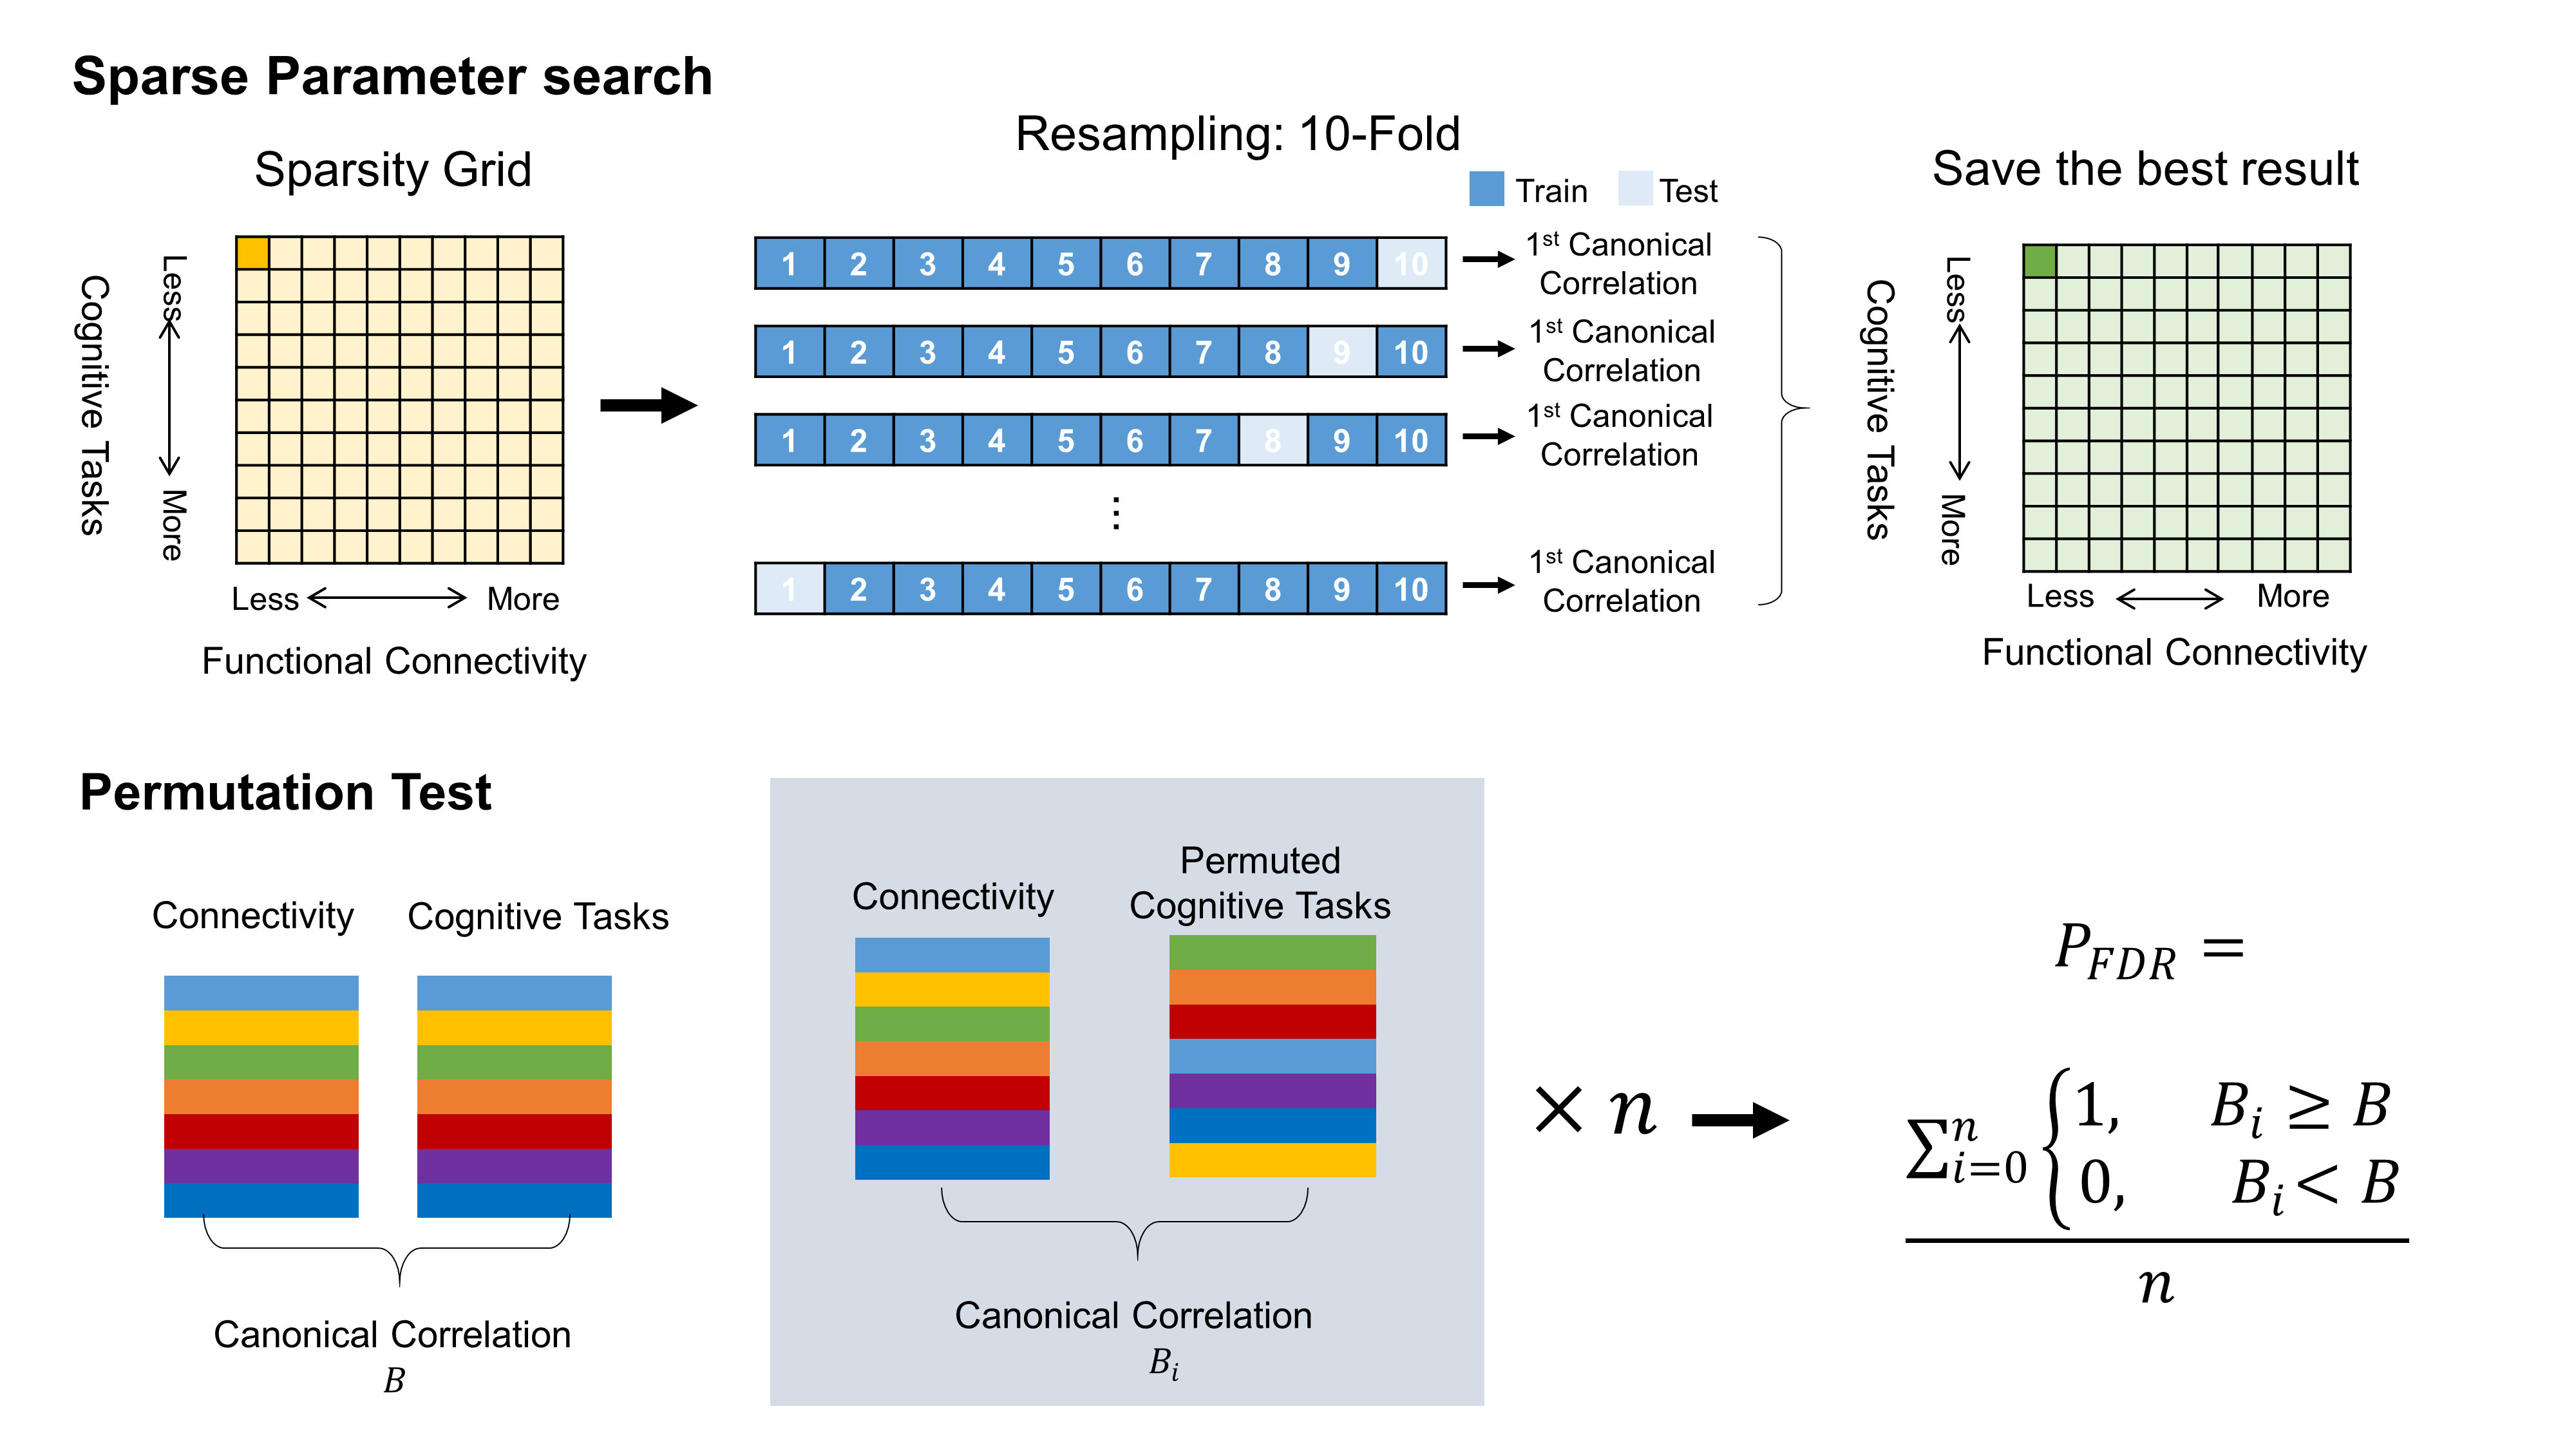
\includegraphics[width=1\textwidth]{study3/image/study3fig1.png}
	\caption{Analysis.}
	\label{fig:study3:fig1}
\end{figure}

\subsection{Group analysis}
\label{study3:method:g}

To determine how patterns of unconstrained neuro-cognitive activity related to performance on the self-report experience summarised in three different ways (see section \ref{study3:method:e:mdes}),
we conducted three independent statistical analysis on the identical subjects. A Type III multivariate multiple regression with Pillai's trace test was applied to the data. Each of the latent components describing the neuro-cognitive mechanism from the SCCA were the independent variables, and the 13 measures from MDES were the dependent variables. We hoped to described the neuro-cognitive components by the linear combination of the self-report questions collected via MDES. The p-values reported were based on Bonferroni correction. The analysis was conducted in R (version 3.3.1). The multivariate multiple regression was conducted in R (version 3.3.1) using function ‘Manova’ in R package ‘car’ (companion to applied regression, version 2.1–5).

% ==========================================================================================================
\section{Results}
\label{study3:results}

\subsection{Determining constituent category of cognitive functions}

Sparse Canonical Correlation Analysis (SCCA) was used to determine connectome-wide dimensions that describe common variance shared by descriptions of brain and experience. This took as input individual scores for the connections between each of the regions extracted from Yeo’s 7 networks parcellation and the 13 cognitive task scores.

\begin{wrapfigure}{o}{0.4\textwidth}
    \vspace{-10pt}
    \centering
    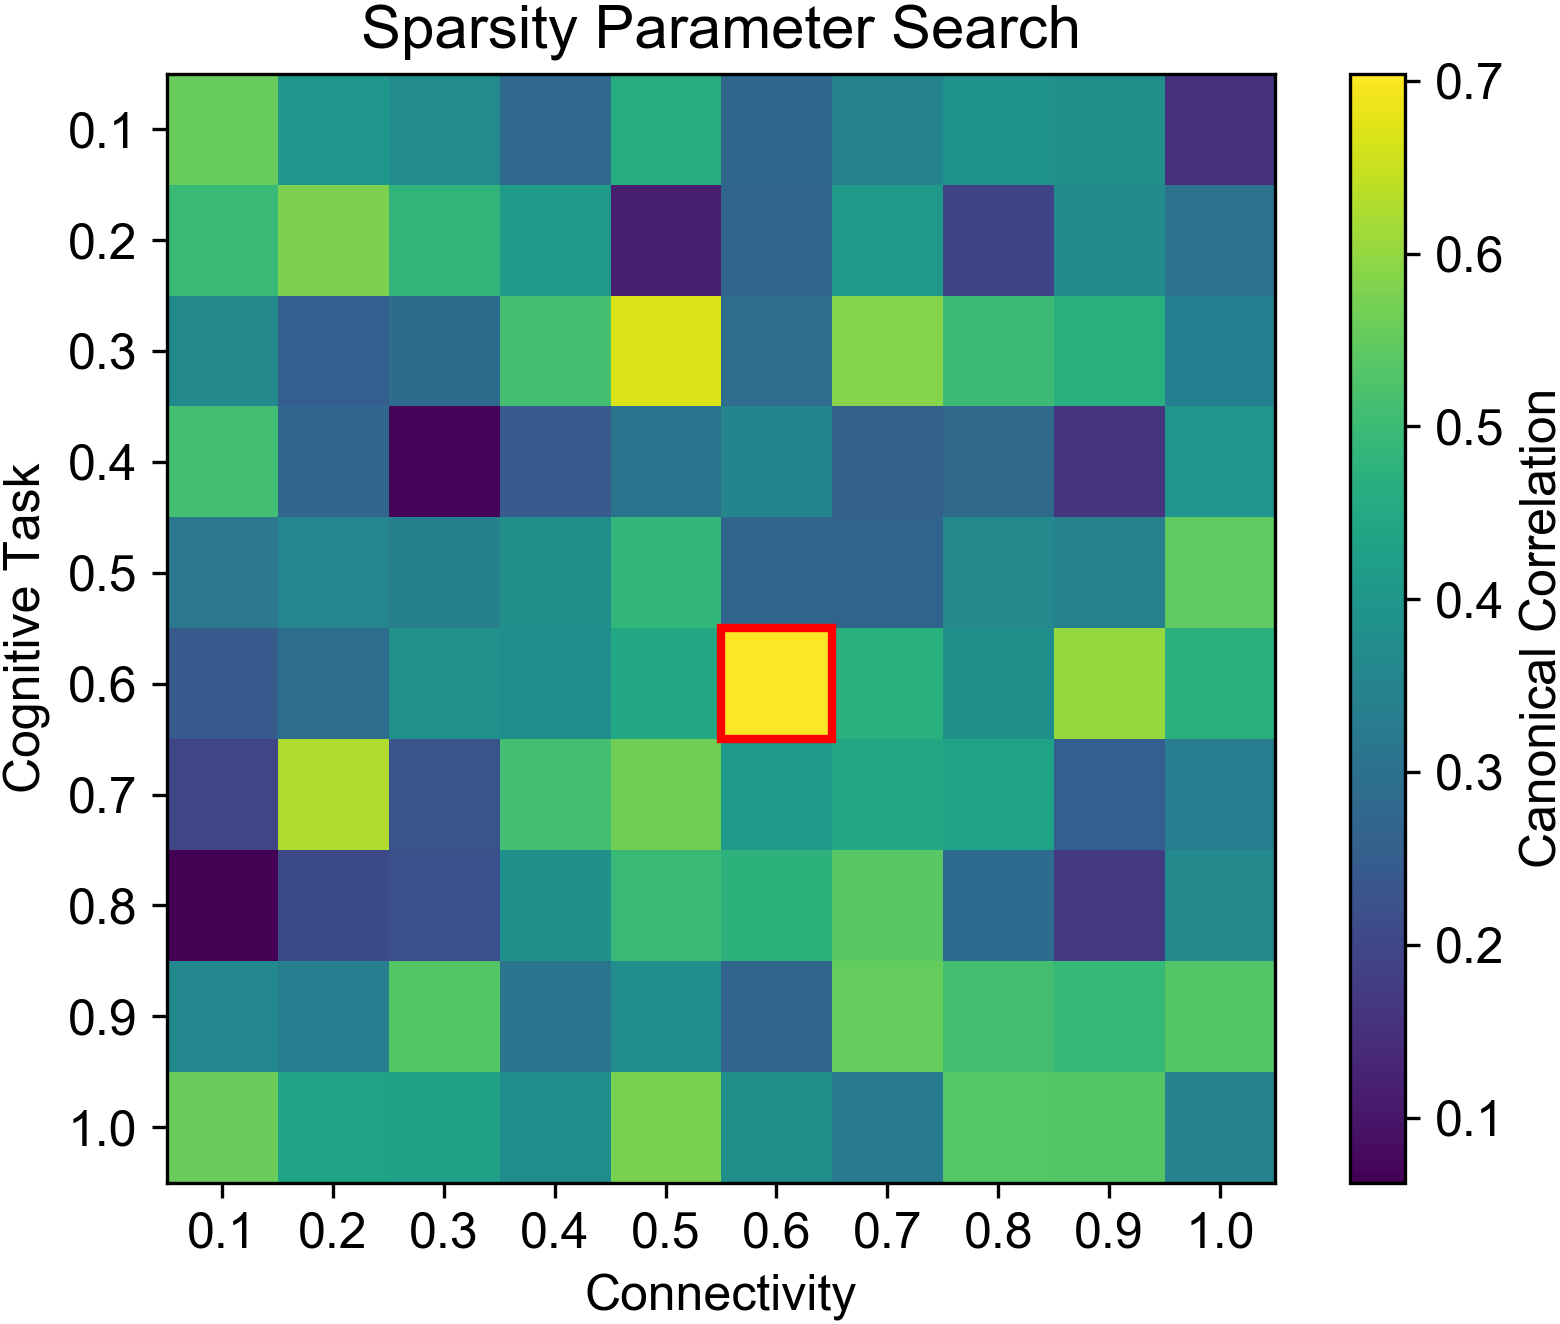
\includegraphics[width=0.38\textwidth]{study3/image/study3fig2.png}
	\caption{Grid search.}
	\label{fig:study3:fig2}
	\vspace{-20pt}
\end{wrapfigure}

We applied SCCA with 10-fold CV and permutation tests as the model selection strategy. We obtained penalty levels of 0.6 on both the functional connectivity and cognitive tasks indicated the best out-of-sample prediction on our data through the grid search (Figure \ref{fig:study3:fig1}), obtaining 0.70 on the rank-1 canonical correlation. Five significant canonical components was identified through FWE-corrected p-value through permutation tests. The p-values of the 5 components are 0.028, 0.042, 0.041, 0.012, 0.033. The canonical correlations of the 5 significant latent components were 0.68, 0.68, 0.68, 0.70, and 0.68. Since the sparsity turns CCA into a convex optimisation problem, the modes didn't come out in the descending order of their canonical correlations.

The latent components yielded by the best model are presented in Figure \ref{fig:study3:fig2}. For the ease of presentation and interpretation, we summarized the components as network-network connectivity instead of 57-by-57 connectivity matrices. The heat maps describe the network-to-network correlations and the cognitive tasks.

\begin{figure}[H]
	\centering
	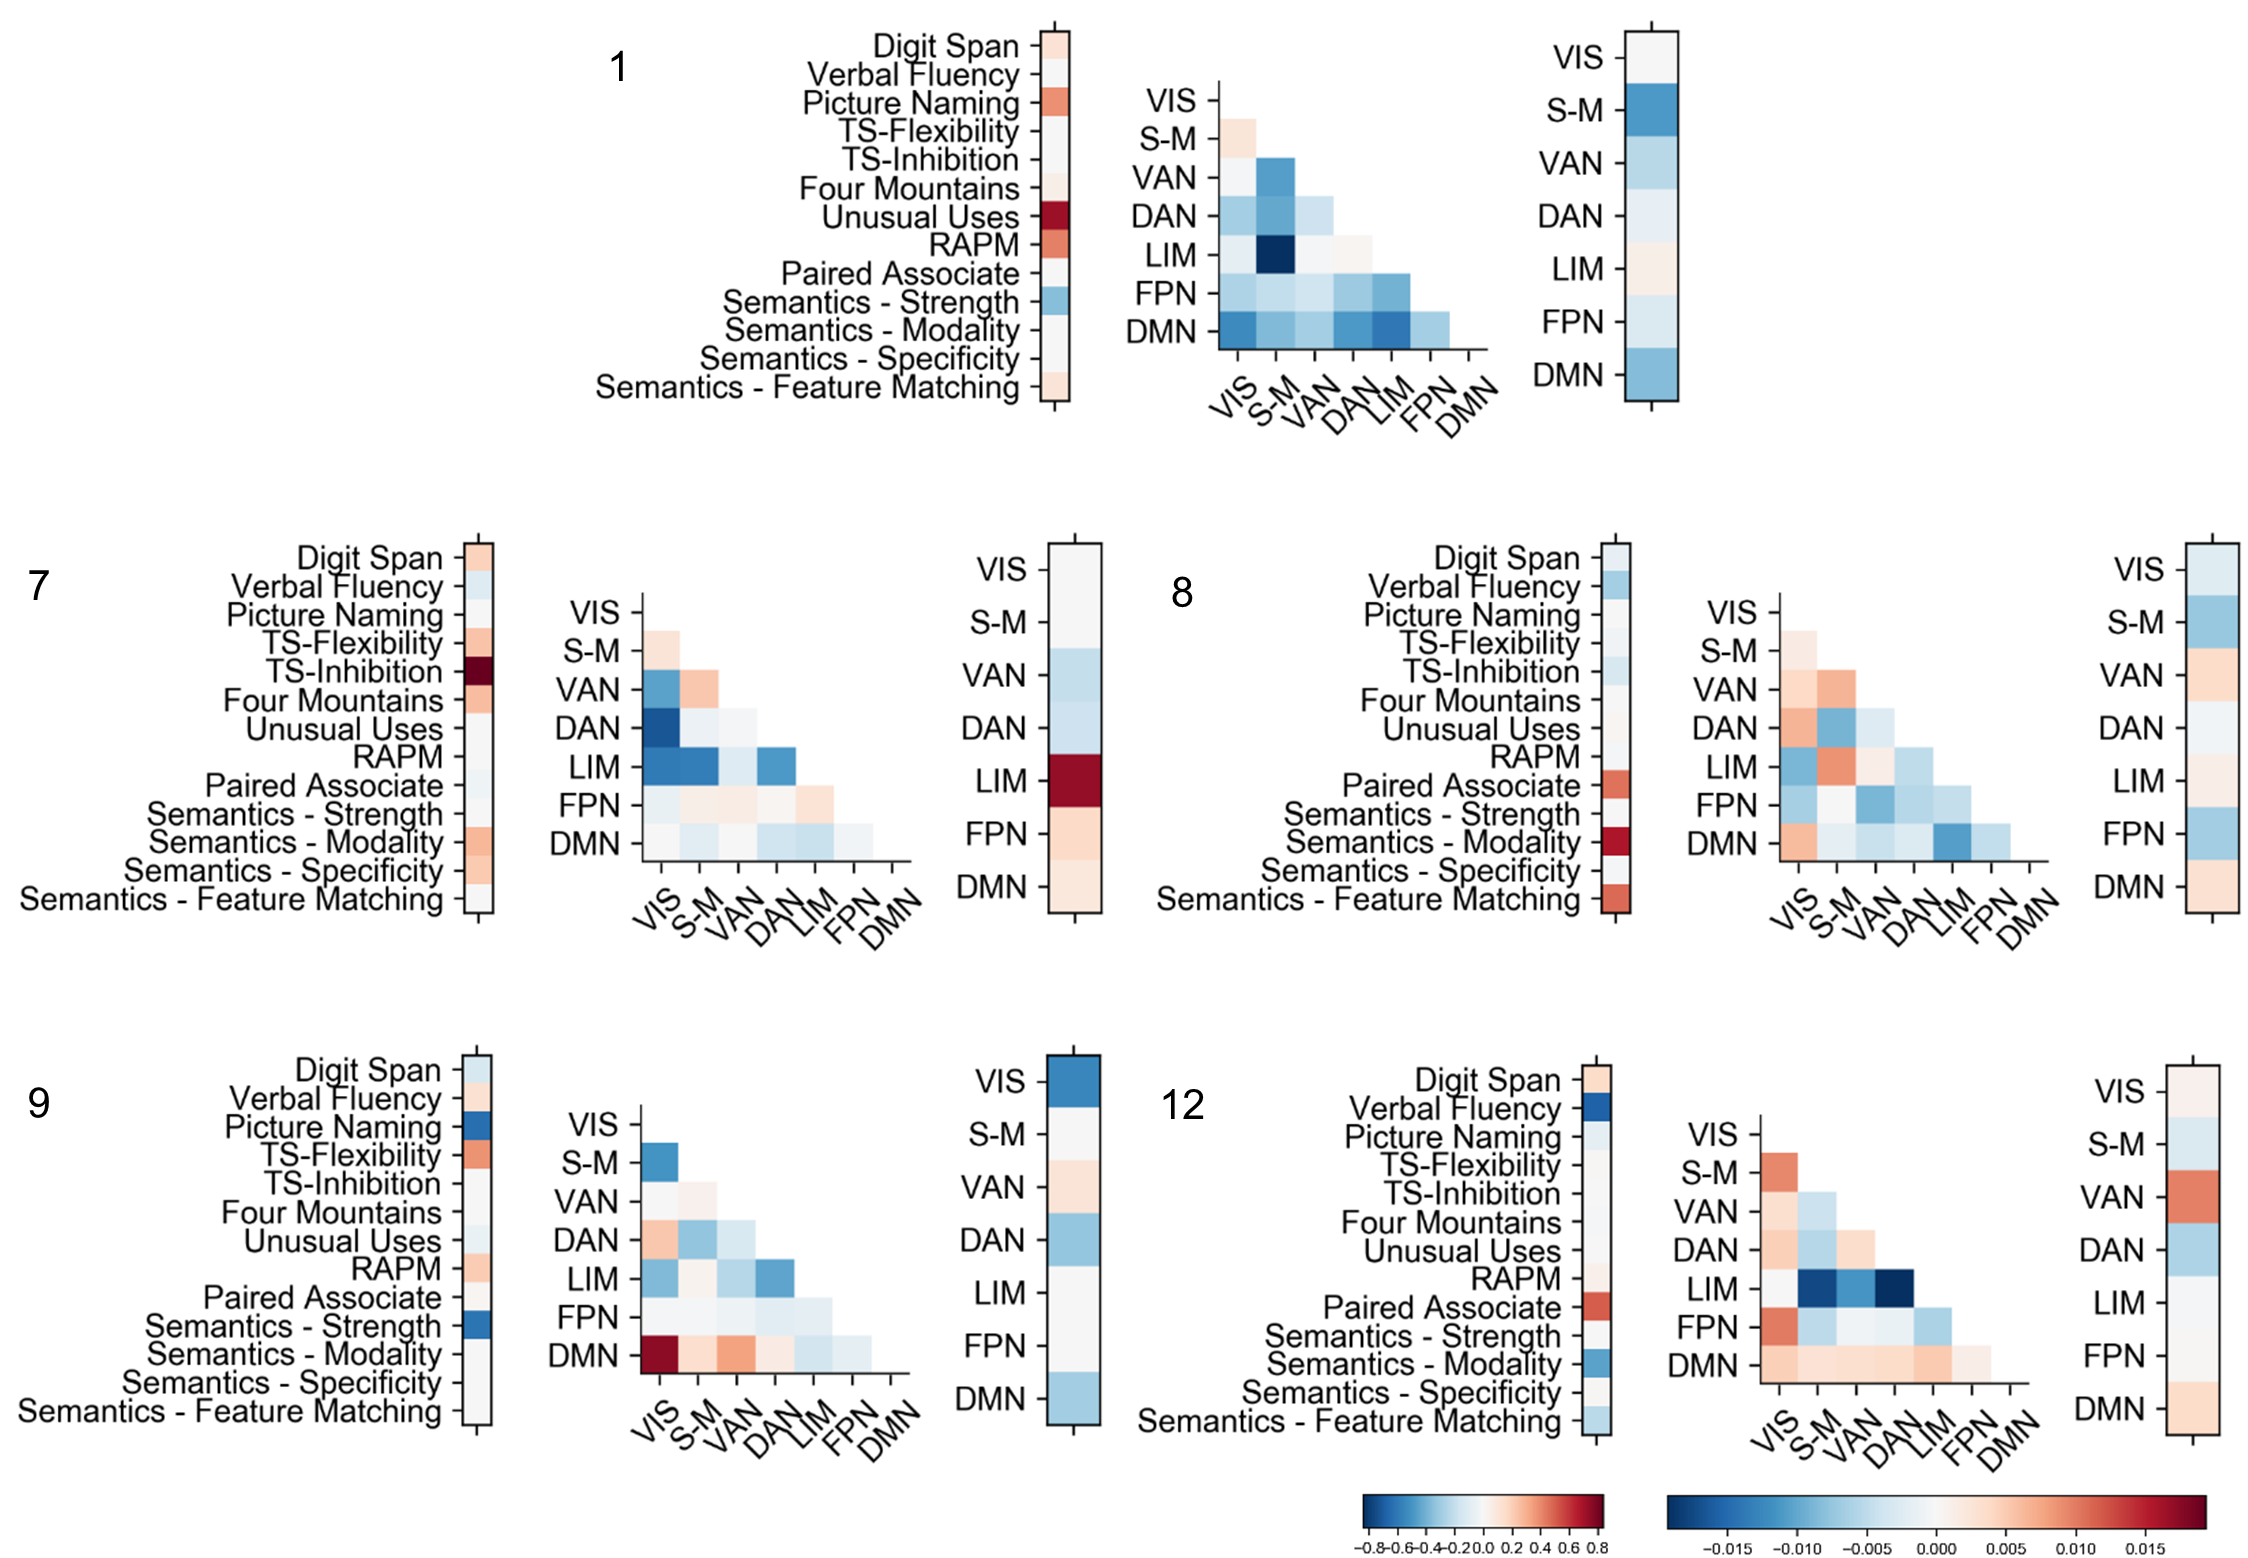
\includegraphics[width=1\textwidth]{study3/image/study3fig3.png}
	\caption{Significant components.}
	\label{fig:study3:fig3}
\end{figure}

% explain the significant components
Component 1 emphasis semantic control with the picture naming task and the unusual uses task, along with intelligence in the cognition component. The negative coefficient in semantic strength indicated the ability to detecting weaker semantics relation. The functional connectivity pattern shows a general dissociation among all networks, especially between the sensorimotor network and the limbic system, and a general dissociation between the unimodal sensory system and the attention and transmodal regions. Component 1 demonstrated semantic control ability to generate mental representation and semantic associations.

Component 7 shows a high coefficient on the inhibition score from the task switching tasks. Specific, imagery related semantic information and tasks related to retaining content such as the four mountains tasks and the digit span task are also relevant. The connectivity pattern showed a dissociation between the sensory input related system and the attention-limbic system. There is also a high connectivity within the regions in the limbic system. Overall, this component demonstrates the ability to be free from other irrelevant sources of information while maintaining a pattern of ongoing thought that is relevant to the original source.

Component 8 put executive tasks against more automatic semantic retrieval. This component demonstrated a strong cognitive control ability. The functional connectivity pattern showed a disassociation among the transmodal systems but high association the between the visual and the attention networks, and between the visual and the attention networks.

Component 9 is composed of tasks involving content generation in a timely manner and   mental imagery, opposing rigid verbal semantic content retrieval. The neural pattern shows a strong correlation between the default mode network and the unimodal systems.

Component 12 highlighted the good episodic memory with the paired associate tasks, and poorer performance on verbal semantic related tasks. The default mode network and visual system showed a general coupling pattern with the whole brain, while a strong dissociation of the limbic with the attention systems and the sensorimotor system. The component demonstrates a strong ability to retain and recall semantically undefined associations.

\subsection{The relationship between neuro-cognitive components and self-reports on thoughts}
% multivariate main effect
Three regression models were performed to evaluate the relationship between neuro-cognitive components and self-reports on thoughts: average scores of all thought probes, thought probes in 0-back and 1-back conditions. In the model of all thought probes, we got multivariate main effect in
component 7 (\textit{F}(13, 160) = 2.239, \textit{p} = .010, \paretasquared = .154)
and 12 (\textit{F}(13, 160) = 1.946, \textit{p} = .029, \paretasquared = .137). There was only one significant univeriate effect after Bonferroni correction,
which is the self question under the model for component 7
(\textit{b} = −0.25, 95\% CI = [−0.40, −0.10], \textit{t}(172) = -3.369, \textit{p} = .005).

In the 0-back condition, only component 7
(\textit{F}(13, 160) = 1.924, \textit{p} = .031, \paretasquared = .135)
showed the main effect in multivaraite level. There was only one significant univeriate effect after Bonferroni correction,
which is the self question under the model for component 7
(\textit{b} = −0.23, 95\% CI = [−0.37, −0.79], \textit{t}(172) = -3.03, \textit{p} = .017).

The 1-back condition model showed significant results in
component 7
(\textit{F}(13, 160) = 2.192, \textit{p} = .012, \paretasquared = .151)
and component 12
(\textit{F}(13, 160) = 2.312, \textit{p} = .008, \paretasquared = .158). There was only significant univeriate effect in the model for component 7 after Bonferroni correction.
The significant variable is the self question
(\textit{b} = −0.26, 95\% CI = [−0.40, −0.11], \textit{t}(172) = -3.51, \textit{p} = .003)
and the habit question
(\textit{b} = −0.22, 95\% CI = [−0.37, −0.75], \textit{t}(172) = -2.97, \textit{p} = .020).

\begin{figure}[H]
	\centering
	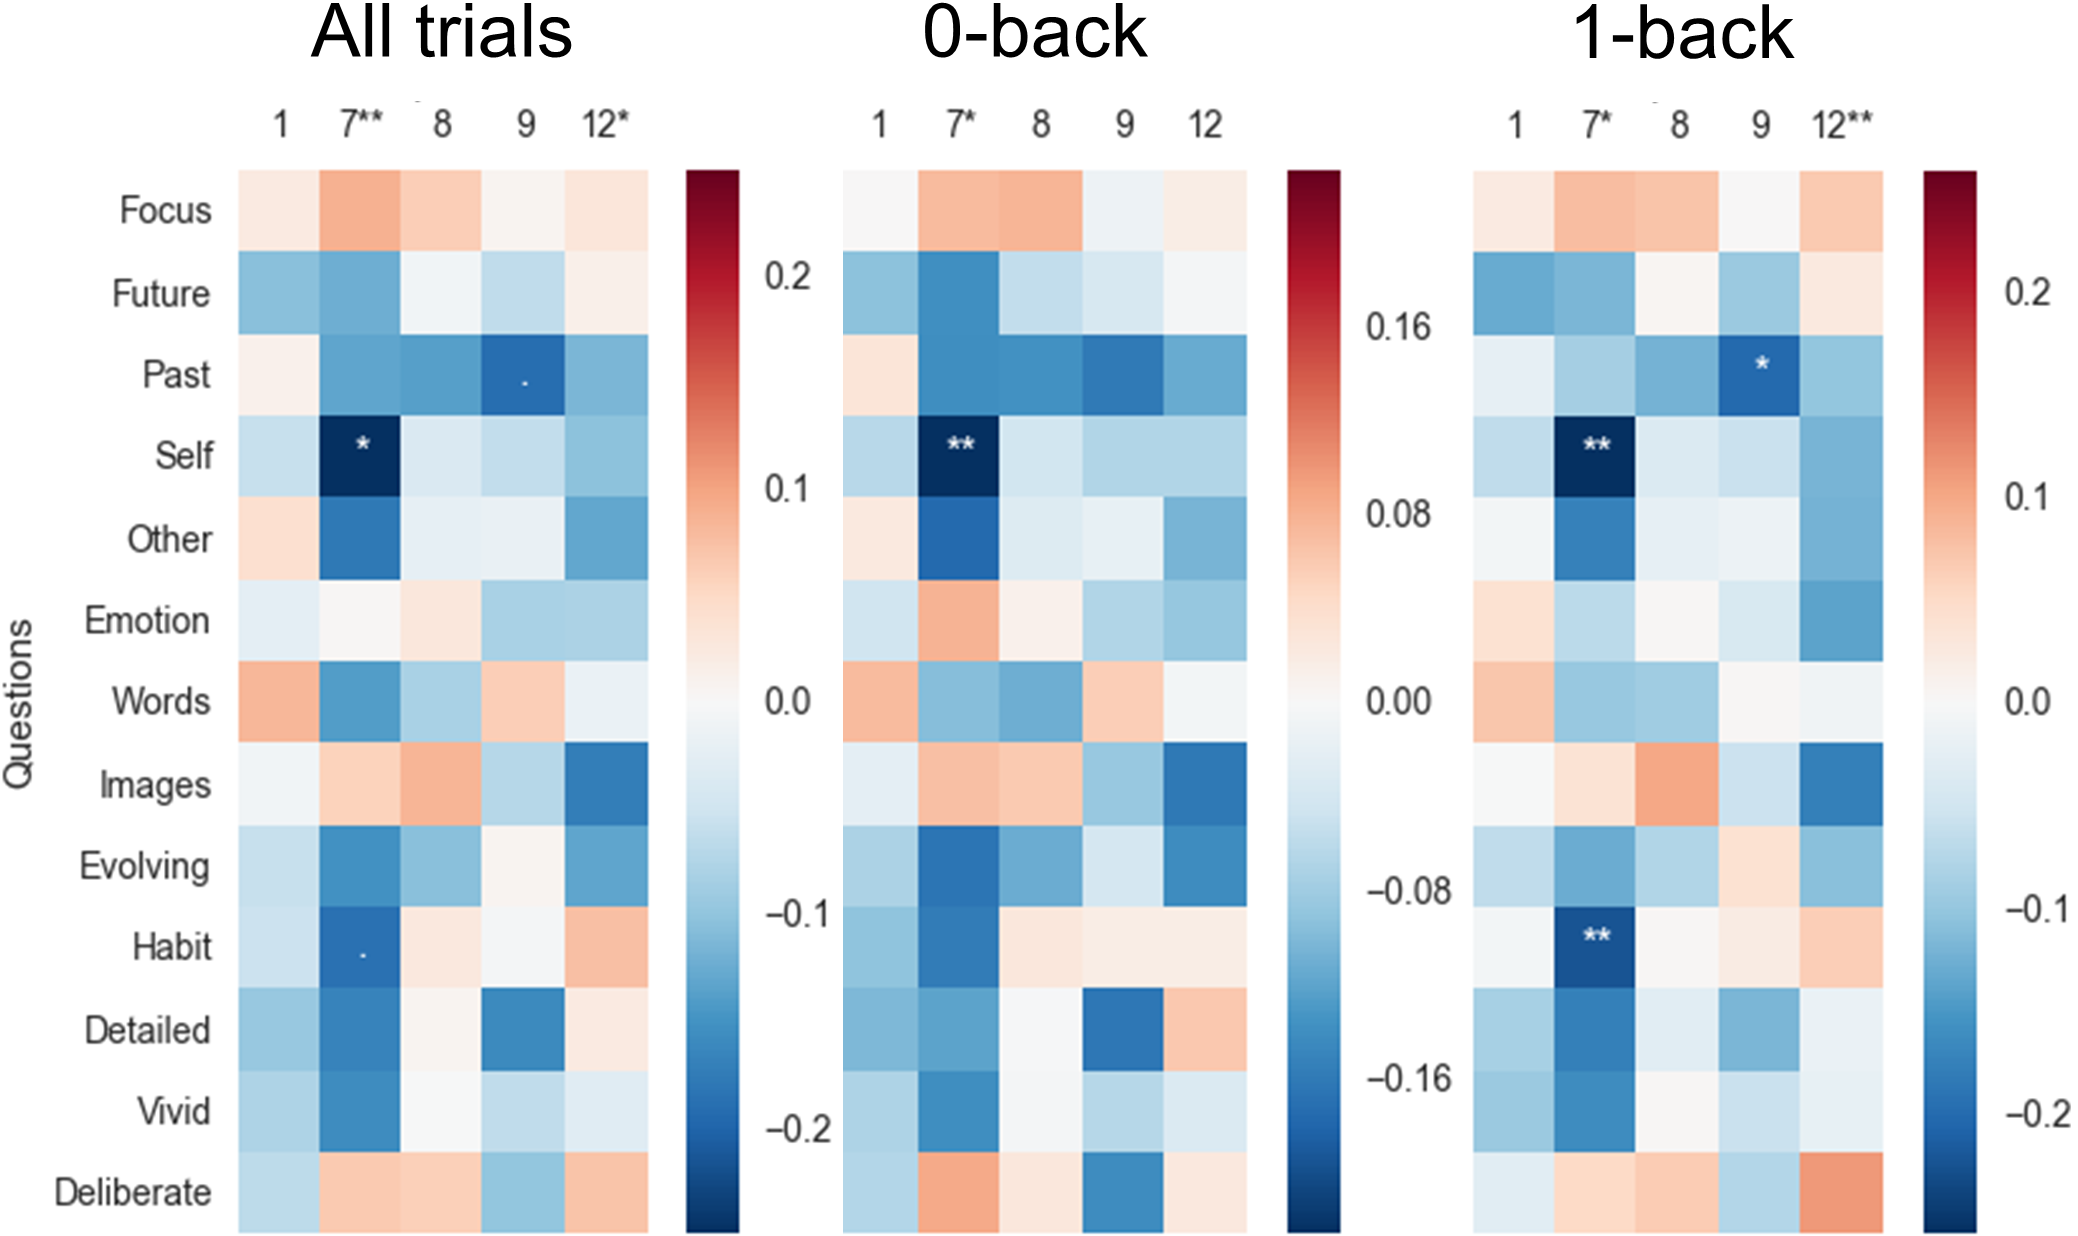
\includegraphics[width=0.8\textwidth]{study3/image/study3fig4.png}
	\caption{Univariate results.}
	\caption*{
	\footnotesize{
	}
	}
	\label{fig:study3:fig4}
\end{figure}


% ==========================================================================================================
\section{Discussion}
\label{study3:discussion}

We set out to identify patterns that described the association between different aspects of cognition and the intrinsic organisation of the cortex, and to explore whether these accounted for variations in patterns of ongoing thought. Using CCA we identified five neuro cognitive dimensions characterized at the cognitive level as creative association, fluid intelligence, temporally specified cognition, and, separate dimensions of episodic memory linked to visual and verbal codes of representation. In our subsequent analysis we identified that variation in temporally specified cognition was associated with substantial variance in patterns of ongoing thought recorded in the laboratory. In particular, we found that this neuro cognitive dimension was associated with variation in both the task relatedness of cognition, and it’s level of immersive details. In the discussion we consider the implications of these data for theoretical accounts of ongoing thought.
In neural terms our CCA analysis suggests that the relative degree of integration / segregation of the limbic system is at the core of whether an individuals experience is a pristine reflection of their current external goal, or instead they are immersed in thoughts generated though imagination. We found that individuals who maintained attention on the task in hand, tended to show a pattern of brain activity dominated by whether the limbic system was coupled to itself, but decoupled from other cortical areas, while individuals who reported off task experiences with immersive qualities showed the reverse pattern (low within network coupling, and high between network coupling for the limbic system). 

These data add to a growing body of evidence that highlight limbic regions as critical for patterns of spontaneous thought. For example, lesions to the hippocampus are associated with reductions in off task thinking (McCormick et al., 2018) and episodic future thinking as part of a task (Maguire et al., 2011; Race et al., 2011). Likewise, semantic dementia, which targets lateral and medial aspects of the temporal pole, reduced the capacity to imagine the future (Irish, et al., 2012; Viard et al. 2014). Furthermore, hippocampus activity has been shown to be important for spontaneous thought during the occurrence of spontaneous thought (Ellamil, et al., 2016), while it’s connectivity with regions of the default mode network are important for both episodic features of spontaneous experience (Karapaganatidis et al., 2017) as well as it’s immersive features (Smallwood et al., 2016). Based on our results, the contribution of limbic structures to spontaneous experience may depend on their coupling with other regions, allowing these hub regions to integrate information from across the cortex to create a mental scene (Hassabis and Maguire). This account is broadly consistent with views of limbic structures, such as the hippocampus (Moscovitch et al., 2016) and the anterior temporal lobe (Lambon-Ralph et al., 2016) which are both thought to share a hub and spoke architecture in which their contribution to cognition arise from their capacity to integrate information from across the cortical mantle. 

In our analysis, participants with whom the limbic system was relatively isolated within the cortical mantle, performed well in a task switching context that required them to suppress representations of a previous task set. Prior uses of this task paradigm have documented that this ability is linked to the tendency to ruminate. Whitmer and colleagues (2007) found that individuals who were high on trait rumination were better than non ruminators when switching back to a prior task. This pattern is broadly consistent with our data which shows that people who show the smallest cost from inhibiting a prior mental set, were more likely to reports patterns of ongoing thought that were characterised by immersive experiences characterised by self relevant, social and episodic content. Building on our study a promising area for future study would be to examine how limbic connectivity supports the recurrence of negative self-relevant experiences that are thought to be important in rumination (Ref). 

Our data suggests that the default mode network shows a similar, albeit less pronounced pattern, to the limbic system. Given evidence of a role for the DMN in both immersive experiences in task states (Sormaz et al., under review, Richter et al., 2015) as well as in off task states (Mason, et al., 2007; Christoff et al., 2009; Stawarkzyck et al., 2010). It is possible that these two networks work in tandem when cognition is focused on self-relevant information with the limbic systems providing the episodic and conceptual content, and the default mode network allowing this content to be represented at a relatively abstract level. This interpretation is consistent with the observation that the default mode network is spatially located at the top of a hierarchy and most distant from unimodal inputs, while limbic regions occupy an intermediate position (Margulies et al., 2016). 

Finally, it is worth considering a number of limitations of this study. First, we did not measure patterns of ongoing thought while individuals performed the battery of cognitive tasks. It is therefore possible that part of the shared variance that our analyses captures emerges because of the patterns of ongoing thought occur during the cognitive tasks (See Mrazek et al., 2012 for evidence of a similar point in the context of executive control or intelligence tasks). However, this interpretation of our data is unlikely since individuals who were off task tended to perform better in the context of the tasks switching task. Second, our neural data was only measured on a single occasion, raising the possibility that this measure of brain function reflects a state rather than a trait. While this remains a possibility, recent studies have shown that individual patterns of functional connectivity remain relatively consistent across tasks and time (Gratton et al., 2018). Nonetheless future studies could benefit from measuring an individuals architecture across multiple points to provide a more robust indication of it’s trait like features. 
